\documentclass{beamer}
\mode<presentation>
\usepackage{amsmath,amssymb,mathtools}
\usepackage{textcomp}
\usepackage{gensymb}
\usepackage{adjustbox}
\usepackage{subcaption}
\usepackage{enumitem}
\usepackage{multicol}
\usepackage{listings}
\usepackage{url}
\usepackage{graphicx} % <-- needed for images
\def\UrlBreaks{\do\/\do-}

\usetheme{Boadilla}
\usecolortheme{lily}
\setbeamertemplate{footline}{
  \leavevmode%
  \hbox{%
  \begin{beamercolorbox}[wd=\paperwidth,ht=2ex,dp=1ex,right]{author in head/foot}%
    \insertframenumber{} / \inserttotalframenumber\hspace*{2ex}
  \end{beamercolorbox}}%
  \vskip0pt%
}
\setbeamertemplate{navigation symbols}{}

\lstset{
  frame=single,
  breaklines=true,
  columns=fullflexible,
  basicstyle=\ttfamily\tiny   % tiny font so code fits
}

\numberwithin{equation}{section}

% ---- your macros ----
\providecommand{\nCr}[2]{\,^{#1}C_{#2}}
\providecommand{\nPr}[2]{\,^{#1}P_{#2}}
\providecommand{\mbf}{\mathbf}
\providecommand{\pr}[1]{\ensuremath{\Pr\left(#1\right)}}
\providecommand{\qfunc}[1]{\ensuremath{Q\left(#1\right)}}
\providecommand{\sbrak}[1]{\ensuremath{{}\left[#1\right]}}
\providecommand{\lsbrak}[1]{\ensuremath{{}\left[#1\right.}}
\providecommand{\rsbrak}[1]{\ensuremath{\left.#1\right]}}
\providecommand{\brak}[1]{\ensuremath{\left(#1\right)}}
\providecommand{\lbrak}[1]{\ensuremath{\left(#1\right.}}
\providecommand{\rbrak}[1]{\ensuremath{\left.#1\right)}}
\providecommand{\cbrak}[1]{\ensuremath{\left\{#1\right\}}}
\providecommand{\lcbrak}[1]{\ensuremath{\left\{#1\right.}}
\providecommand{\rcbrak}[1]{\ensuremath{\left.#1\right\}}}
\theoremstyle{remark}
\newtheorem{rem}{Remark}
\newcommand{\sgn}{\mathop{\mathrm{sgn}}}
\providecommand{\abs}[1]{\left\vert#1\right\vert}
\providecommand{\res}[1]{\Res\displaylimits_{#1}}
\providecommand{\norm}[1]{\lVert#1\rVert}
\providecommand{\mtx}[1]{\mathbf{#1}}
\providecommand{\mean}[1]{E\left[ #1 \right]}
\providecommand{\fourier}{\overset{\mathcal{F}}{ \rightleftharpoons}}
\providecommand{\system}{\overset{\mathcal{H}}{ \longleftrightarrow}}
\providecommand{\dec}[2]{\ensuremath{\overset{#1}{\underset{#2}{\gtrless}}}}
\newcommand{\myvec}[1]{\ensuremath{\begin{pmatrix}#1\end{pmatrix}}}
\let\vec\mathbf

\title{MatGeo Presentation - Problem 1.6.14}
\author{EE25BTECH11064 - Yojit Manral}
\date{}

\begin{document}

\frame{\titlepage}
\begin{frame}{Question}
For which values of a and b does the following pair of linear equations have an infinite number of solutions?
\begin{align*}
    2x + 3y &= 7 \\
    (a - b)x + (a + b)y &= 3a + b - 2
\end{align*}
\end{frame}

\begin{frame}{Solution}
$\rightarrow$ The equation of the lines can be written as
\begin{align}
    \vec{n_1}^{T}\vec{x} &= c_1 \\
    \vec{n_2}^{T}\vec{x} &= c_2
\end{align}
\hspace{0.3cm} where,
\begin{align}
    \vec{n_1} &= \myvec{2\\3} \\
    \vec{n_2} &= \myvec{a-b\\a+b} \\
    c_1 &= 7 \\
    c_2 &= 3a + b -2
\end{align}
\end{frame}

\begin{frame}{Solution}
$\rightarrow$ For two lines to have infinite solutions,,
\begin{align}
    \vec{n_1} &= \alpha \vec{n_2} \\
    c_1 &= \alpha c_2 \\
    \implies c_2 \vec{n_1} &= c_1 \vec{n_2}
\end{align}
$\rightarrow$ Substituting the values from (3), (4), (5), and (6) in (9)
\begin{align}
    (3a + b - 2)\myvec{2\\3} &= 7 \myvec{a-b\\a+b} \\
    \myvec{6a + 2b\\9a + 3b} - \myvec{7a-7b\\7a+7b} = \myvec{-a + 9b\\2a - 4b} &= \myvec{4\\6} \\
    \implies \myvec{-1&&9\\2&&-4}\myvec{a\\b} &= \myvec{4\\6}
\end{align}
\end{frame}

\begin{frame}{Solution}
$\rightarrow$ Using row transformations
\begin{align}
    \myvec{-1&&9\\2&&-4}\myvec{a\\b} = \myvec{4\\6} &\xrightarrow{R_1 \leftrightarrow -R_1} \myvec{1&&-9\\2&&-4}\myvec{a\\b} = \myvec{-4\\6} \\
    &\xrightarrow{R_2 \leftrightarrow R_2 - 2R_1} \myvec{1&&-9\\0&&14}\myvec{a\\b} = \myvec{-4\\14} \\
    &\xrightarrow{R_2 \leftrightarrow (1/14)R_2} \myvec{1&&-9\\0&&1}\myvec{a\\b} = \myvec{-4\\1} \\
    &\xrightarrow{R_1 \leftrightarrow R_1 + 9R_2} \myvec{1&&0\\0&&1}\myvec{a\\b} = \myvec{5\\1} \\
    \implies &\myvec{a\\b} = \myvec{5\\1} \implies a = 5 \text{ and } b = 1
\end{align}
\end{frame}

\begin{frame}{Solution}
\begin{figure}[h!]
   \centering
   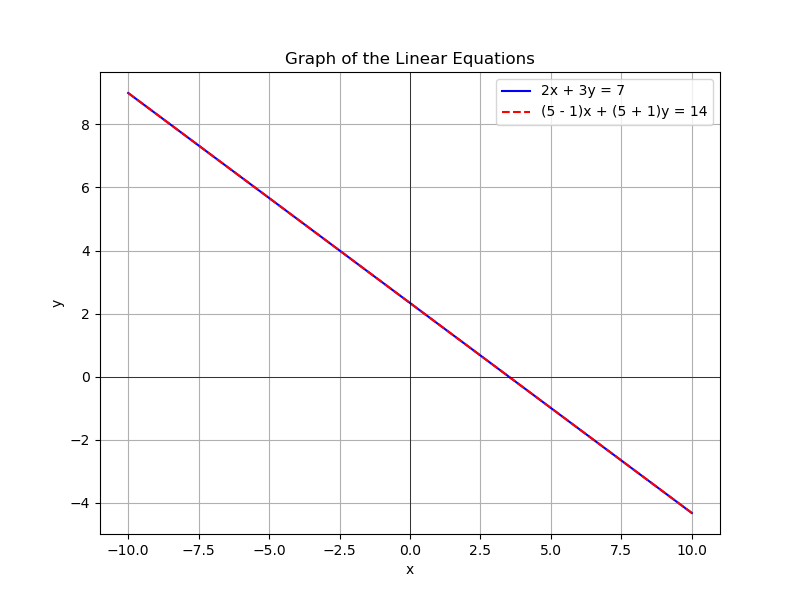
\includegraphics[width=0.8\linewidth]{figs/01.png}
   \caption{Plot of the lines}
   \label{Plot_1}
\end{figure}
\end{frame}
 % --------- CODE APPENDIX ---------
\section*{Appendix: Code}
% Python plotting
\begin{frame}[fragile]{File: plot.py}
\begin{lstlisting}[language=Python]
import numpy as np
import matplotlib.pyplot as plt

# Set the values of a and b
a = 5
b = 1

# Define the equations
def line_eq1(x):
    return (7 - 2*x) / 3  # y = (7 - 2x) / 3

def line_eq2(x, a, b):
    return (3*a + b - 2 - (a - b)*x) / (a + b)  # y = (3a + b - 2 - (a - b)x) / (a + b)

# Generate x values
x_vals = np.linspace(-10, 10, 400)

# Calculate the corresponding y values for both lines
y_vals_eq1 = line_eq1(x_vals)
y_vals_eq2 = line_eq2(x_vals, a, b)
\end{lstlisting}
\end{frame}

\begin{frame}[fragile]{File: plot.py}
\begin{lstlisting}[language=Python]
# Plot the lines
plt.figure(figsize=(8, 6))
plt.plot(x_vals, y_vals_eq1, label="2x + 3y = 7", color="blue")
plt.plot(x_vals, y_vals_eq2, label=f"({a} - {b})x + ({a} + {b})y = {3*a + b - 2}", color="red", linestyle="--")

# Add labels and title
plt.xlabel('x')
plt.ylabel('y')
plt.title('Graph of the Linear Equations')
plt.axhline(0, color='black',linewidth=0.5)
plt.axvline(0, color='black',linewidth=0.5)

# Add a legend
plt.legend()

# Show the plot
plt.grid(True)
plt.show()

\end{lstlisting}
\end{frame}
\end{document}
